\documentclass[12pt, letterpaper, titlepage]{article}

\usepackage{amsmath, amsfonts}
\usepackage{booktabs}
\usepackage{amsthm}
\usepackage{graphicx}
\usepackage[margin=1in]{geometry}
\usepackage{hyperref}
\usepackage{cleveref}
\hypersetup{colorlinks = true, linkcolor = blue, citecolor=blue, urlcolor = blue}
\usepackage{natbib}
\usepackage{float}
\usepackage{setspace}
\usepackage{pdfpages}
\usepackage[pagewise]{lineno}
\usepackage{mwe}
\usepackage{comment}
%\linenumbers*[1]
% %% patches to make lineno work better with amsmath
\newcommand*\patchAmsMathEnvironmentForLineno[1]{%
 \expandafter\let\csname old#1\expandafter\endcsname\csname #1\endcsname
 \expandafter\let\csname oldend#1\expandafter\endcsname\csname end#1\endcsname
 \renewenvironment{#1}%
 {\linenomath\csname old#1\endcsname}%
 {\csname oldend#1\endcsname\endlinenomath}}%
\newcommand*\patchBothAmsMathEnvironmentsForLineno[1]{%
 \patchAmsMathEnvironmentForLineno{#1}%
 \patchAmsMathEnvironmentForLineno{#1*}}%

\AtBeginDocument{%
 \patchBothAmsMathEnvironmentsForLineno{equation}%
 \patchBothAmsMathEnvironmentsForLineno{align}%
 \patchBothAmsMathEnvironmentsForLineno{flalign}%
 \patchBothAmsMathEnvironmentsForLineno{alignat}%
 \patchBothAmsMathEnvironmentsForLineno{gather}%
 \patchBothAmsMathEnvironmentsForLineno{multline}%
}

% control floats
\renewcommand\floatpagefraction{.9}
\renewcommand\topfraction{.9}
\renewcommand\bottomfraction{.9}
\renewcommand\textfraction{.1}
\setcounter{totalnumber}{50}
\setcounter{topnumber}{50}
\setcounter{bottomnumber}{50}

\newcommand{\jy}[1]{\textcolor{blue}{JY: #1}}
\newcommand{\eds}[1]{\textcolor{red}{EDS: (#1)}}
\newcommand{\of}[1]{\textcolor{violet}{OF: #1}}


\title{On Devon Allen's Disqualification at the 2022 World Track and Field 
Championships} 

\author{Owen Fiore\\
%   \href{mailto:owen.fiore@uconn.edu}
% {\nolinkurl{owen.fiore@uconn.edu}}\\
  Elizabeth Schifano\\
  Jun Yan\\[1ex]
  Department of Statistics, University of Connecticut\\
}
\date{}

\begin{document}
\maketitle

%Abstract should be 200 words
%Devon Allen was disqualified in 2022... discussions about dq, talk methods and 
%models, venue effect, and conclusion
\begin{abstract}
Devon Allen was disqualified in the men's 110 meter hurdle final of the 2022
World Track and Field Championships after registering a reaction time of 0.099 
seconds, 0.001 seconds faster than what is allowed. Following the games, 
bloggers on the running website LetsRun concluded that the reaction time data 
from the 2022 World Championships seemed to be generally faster compared to the 
other datasets they considered, but they did not perform any formal 
statistical analyses. This paper questions the reaction time 
disqualification barrier, which is currently 0.1 seconds, to determine whether 
this is a reasonable threshold. We employ a generalized linear mixed model 
(GLMM) with a random venue effect in order to  model the reaction time data. 
Additionally, we employ a signed-rank test for clustered data to 
compare reaction times for the same athletes at different competitions. This 
matter needs to be addressed because disqualification based on allowable 
reaction time will continue to be an issue in future world championships.




\bigskip\noindent{\sc Keywords}:
False Start, Hurdles, Reaction Time, Seiko 

\end{abstract}

\doublespace

\jy{The bib file needs quality control. Practice my writing tips in the
  stat-wriging notes: chapter 2 on latex/bibtex.}

\jy{Go over the reference section to see what need to be changed in the bib source}

\section{Introduction}
\label{sec:intro}


Devon Allen, an alumnus of the University of Oregon in 
Eugene, Oregon, was
expected to be a contender for the 2022 World Track and Field Championships 110 
meter hurdle.  After running the event in 12.84 seconds in early June 2022 
(only 0.04 seconds away from the world record \citep{wa2022preview}) and coming 
in third at the United States Track and Field 
Championships also in Eugene in late June, Allen was poised to compete in the 
2022 World Track and Field Championships at the same Eugene venue in August.
At the World Championships, Allen made it through the preliminary
heats and semifinals to reach the final heat while posting reaction times of 
0.123 and 0.101 in his preliminary heat and semifinal, respectively.  
His disqualification in the final heat by reacting in 0.099 seconds instead of 
0.1 was met
with shock from both Allen and fans alike.  NBC, who was broadcasting the
championships in the United States, later uploaded a video to their YouTube
channel that showed the disqualification
(\url{https://www.youtube.com/watch?v=D6NXTMo-1yM}).
The crowd erupted with jeers
when they found out that Allen was disqualified, angry at the result.  Had Allen 
reacted just 0.001 seconds slower he would have been allowed to compete and been 
spared waiting until the next World Track and Field Championships.

%2)
Allen's disqualification has been discussed extensively in online communities
such as \url{www.LetsRun.com}, a website that is part message board and part
news. The message board,
which functions similarly to Reddit, is very active during important running
events, including during the finals of major events such as
the Olympics and the World Track and Field Championships.  However, it is the
news section of the website that generated articles such as \citet{johnson2022data}
and \citet{johnson2022was} from  Robert Johnson, who created and runs 
the LetsRun website.  He argued that there was an error
with the timing equipment at the 2022 World Track and Field Championships and
cited graphs, computed simple statistics such as median reaction times, and 
compared the reaction times at the 2022 World Track and Field Championships to 
other competitions
such as the United States Track and Field Championships and other World Championships.
The comparisons lacked formal statistical analysis, however. 
The alleged 99.95\% chance Allen was wronged 
came from Johnson claiming there is a $(1/13)^3$ chance that the fastest 
reaction times over the past 13 competitions of the men's 100 meter, men's 110 
meter hurdle, and women's 100 meter would all come from the same year 
\citep{johnson2022was}.


\jy{Use double blank lines to separate paragraphs in tex source}

Reaction time in sprint and hurdle events has been studied by many authors.
\citet{pain2007sprint} examined
reaction times for nine male athletes.  The
fastest athlete of the nine had, on average (even with their two fastest times 
removed), a reaction time of 0.087 seconds and a standard deviation of 0.004
seconds.  Two other athletes were able to react similarly when under certain
muscular tightening conditions \citep{pain2007sprint}. 
In a study commissioned by International Association of Athletics Federations 
(IAAF), \citet{komi2009iaaf} recommended that the disqualification 
barrier be decreased to allow sprinters to
react faster, and suggested 0.08 or 0.085 seconds as possible new thresholds.
Additionally, it was recommended to IAAF that high speed cameras be used to
change the reaction time criteria from pushing off on the block to body
movement. This could provide a more accurate representation of reaction time, 
and thus the possibility of a false disqualification would be lowered.
The possibility of using a video-based medium has been proved to be a reliable
measure of reaction time \citep{mudric2015evaluation}.


\citet{pilianidis2012start} found
significant differences between reaction times at several world championships
between 1997 and 2009 for the men's 110 meter hurdles.  Another important
conclusion was that reaction times did not decrease over the twelve years
covered by the research in the study \citep{pilianidis2012start}. This 
contradicts the results of \citet{zhang2021correlation}, which indicated that 
year of competition has a significant effect on reaction times.  Their
analysis looked at data from the 2011-2019 World Championships across multiple
sprint events and concluded that from 2011 to 2019, reaction times got
faster. However, not all studies have been in favor of a decrease in the
reaction time barrier. \citet*{brosnan2017effects} argue for increasing 
the reaction time barrier to 0.115 seconds, and cited evidence from European 
Championships and World Championships in their article.  A study looking 
at the 2008 Olympics likewise supported the conclusion that athletes could not
react in as little as 0.1 seconds \citep{lipps2011implications}.  Another study
concluded that visual reaction times to the starting gun may be faster by 0.007
seconds than the IAAF method, which is from force on block starts 
\citep{holmes2018method}.  While this may seem trivial, Allen was disqualified
only by 0.001 seconds. It is also worth noting that one study looking at data 
from various IAAF meets found that the fastest reaction times for men were found
between the ages of 26 and 29 \citep{tonnessen2013reaction}.  This is notable 
because Allen was 27 years old at the 2022 World Track and Field Championships 
and likely at his physical peak.


\jy{This paragraph reads disconnected. Should it be merged with paragraph~3
  where the study was reviewed?}
Despite their study, IAAF has not changed the reaction barrier since it was
implemented at the 1999 World Track and Field Championships.  It is unclear
why IAAF would commission a study only to disregard the results and not
make the recommended changes.  It is unknown how many athletes since 2009 could
have potentially benefited from this, but it is probable that there are others
besides Allen who were disqualified.


The objective to this paper is to analyze the reaction times at the 2022 World 
Track and Field Championships to check for any abnormalities, and we approach
this in two different ways.  First we model the data, which are
the reaction times of every non-disqualification since the 1999 World 
Championships, using a gamma linear mixed-effects model with a random effect 
accounting for the venue (or year). 
Based on the fitted model, we can then estimate the probability of a reaction 
time being below a certain threshold (e.g., 0.1). 
Second, we compare reaction times for athletes who have competed
at additional competitions to the 2022 World Track and Field Championship.  By
comparing reaction times from the same athlete across multiple competitions we 
are able to determine if the 2022 reaction times differed significantly from 
those of other competitions.
Our investigation into reaction times is important not only because of its
implications for future races, but also because reaction times have
been shown to affect the overall time of the race \citep{delalija2008reaction}.
Thus, faster reaction times lead to faster overall times, which is the goal of
every sprinter who steps onto the track.


The rest of this paper is organized as follows. Section~\ref{sec:Data} describes 
how data was collected and begins to detail the generalized linear mixed-effect 
(GLMM) model that is further developed in Section~\ref{sec:Methods}. The 
signed-rank test that analyzes reaction times for the same athletes across
different competitions is
also described in Section~\ref{sec:Methods}.  Section~\ref{sec:Results}
 provides the results of the two analyses and ends 
by questioning the reaction time barrier.  Lastly, Section~\ref{sec:Discussion}
discusses the impact and limitations of the paper.


\section{Data} \label{sec:Data}

There are two types of data that are explored throughout this paper: data from
1999-2022 for every world championship, and data from athletes who competed in
the 2022 World Championships and another competition (either 2019 World 
Championships or a 2022 national competition typically held within three months 
of the 2022 World Championships). 
\eds{is this true? are you still using the 2019 world championships data for the
rank-based analyses, or only the national competitions?}
\of{Yes the ranked based comparison has 2 subsections: 2022 national vs 2022
international and 2019 international vs 2022 international.  Should I instead say
that there are three types of data across 2 sections or something like that?}
\eds{I think this is fine here, but it is not at all clear that there are two
subsections in the rank-based results for 2022 national vs 2022
international and 2019 international vs 2022 international.}
\of{Currently under the Methods/Results section I have GLMM and rank based comparison
do you think I need subsections under rank based comparison, or is that too much
compartmentalization?  Or should I instead say there are 3 types of data that are
used in two different methods, or something like that?} \eds{I prefer
subsections within rank-based comparison.}
The first data set is used for the GLMM analyses described in 
Section~\ref{sec:glmm}, while the second collection of data is used for the 
rank-based comparisons described in Section~\ref{sec:rank}.

\subsection{World Championships}\label{sec:dataworld}


\begin{figure}[tbp]
  \centering
  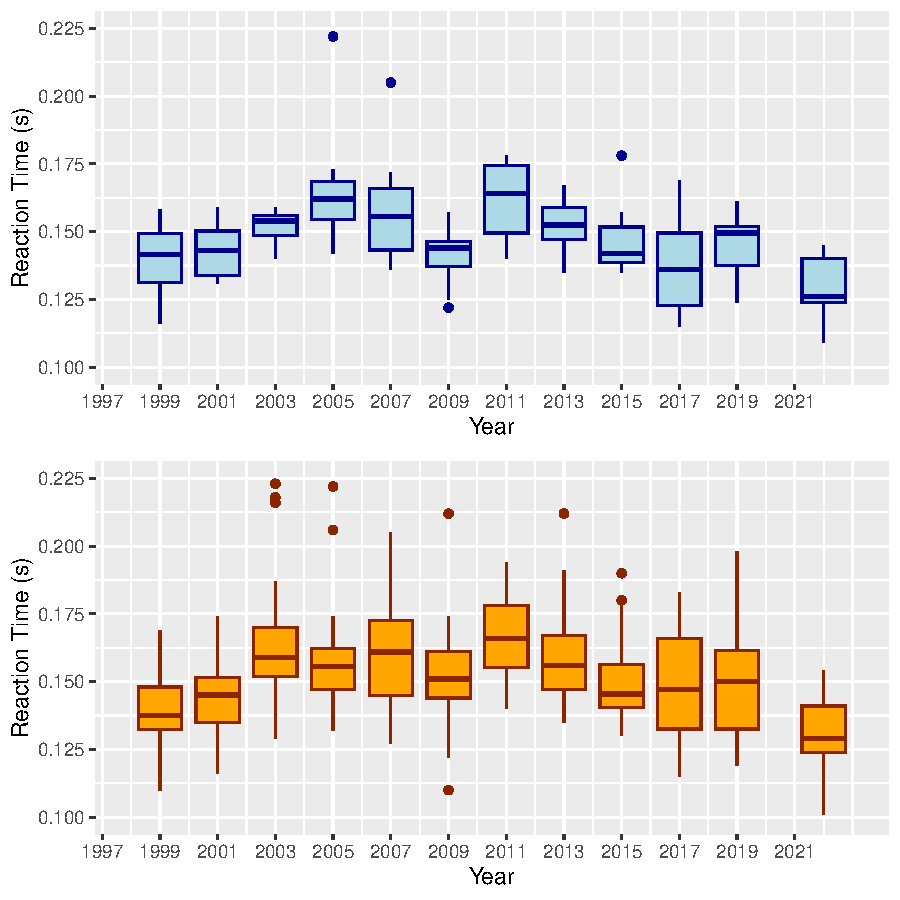
\includegraphics{Finals_Pooled_Boxplot}
  \caption{The reaction times from 1999 to 2022 for the men's final (top) and
  the men's semifinals and finals (bottom).}
  \label{fig:Boxplots}
\end{figure}


Data was taken from the World Athletics 
and covers the men's 110 meter hurdles from 1999 to 2022; the source can be 
found in the Appendix.
Although women's data is available, we chose not to include women's data in the
analyses to follow due to the numerous papers citing differences in men and
women's reaction times \citep[e.g.,][]{lipps2011implications, 
babicc2009reaction, panoutsakopoulos2020gender}.
We focus on the reaction times during the semifinal and final heats only, as 
reaction times from preliminary heats are often not as fast as those in later 
heats \citep[e.g.,][]{zhang2021correlation}. 

For analysis purposes, we will often pool reaction times of men's final and 
men's semifinal heats together and refer to this data as the ``pooled data"
throughout the paper. 
%\of{Ok I updated this.  Should I delete the batch variable too?  Although I don't
%use it, I do reference it in the methods section}
The pooled data increases the sample size which is advantageous because in some
years there are very few final heat observations.  For example, in 2022 there
were only five data points due to two disqualifications and one athlete who 
did not compete.  We also look at data that does not include 2022 with year values
between 1999 and 2019.  Thus, we have four datasets with their respective naming
in parentheses: the final's data from 1999 to 2019 (Old Finals), final's data 
from 2019 to 2022 (All Finals), pooled data from 1999 to 2019 (Old Pooled), and 
pooled data from 1999 to 2022 (All Pooled).

The data under consideration is best visualized using side-by-side boxplots, as
shown in Figure~\ref{fig:Boxplots}.  It is clear that the reaction times in the 
2022 boxplot for both 
the men's finals and men's pooled semifinal and final data are lower (indicating 
faster reaction times)
than in previous years.  The median for the men's pooled data in 2022 was 0.129
and the median for the men's final data in 2022 was 0.126.  For comparison,
\citet{brosnan2017effects} found median reaction times of 0.156 seconds 
for men when looking at data from 1999 to 2014.

We can also see from Figure~\ref{fig:Boxplots} that the reaction times clearly
differ from year to year. The venue of the World Championships changes each 
year, so weather or climate related factors such as humidity, precipitation, 
elevation, may indeed play a role, but additionally, both the technology and 
false start penalization rules have changed over the study period.

From 2007--2009, the IAAF (the former name for World Athletics, and the 
governing body for the World Track and Field Championships) instituted a rule 
change that allowed one warning false start before a sprinter was disqualified 
\citep{iaaf2009falsestart}. There were 18 male and 7 female false starts at the 
2007 World Championships, and 18 male and 7 female false starts at the 2009 World 
Championships. Starting in 2011, the rule was scrapped, and the old policy which
automatically disqualifies runners who false start was reinstated. This was 
desirable for World Athletics as false starts can make already lengthy track 
meets more tedious, both for athletes and viewers watching the television 
broadcast. By returning to the harsher policy and cracking down on false starts,
World Athletics had reduced men's false starts by two thirds in 2011 (6 male and
4 female disqualifications) \citep{iaaf2009falsestart}. \citet{haugen2013effect}
examined the effect of different false start rules that IAAF has imposed from 
1997 to 2009 and found statistically significant improvement in reaction times 
under more lenient rules.




\subsection{Beyond World Championships}\label{sec:databeyond}
The motivation for looking beyond World Championships data came from an 
exploratory analysis examining how United States athletes reacted at the 
2022 United States Track and Field Championships.

From June 23-26 2022, the United States held its Track and Field Championships 
at Hayward Field in Eugene, Oregon to decide who to send to the World Championships 
being held at the same venue in August. Thus, we can establish a baseline for the four United States athletes who 
competed in at least one round of both events: Trey Cunningham, Daniel Roberts, 
Grant Holloway, and Devon Allen. Every athlete reacted faster in all the World 
Track and Field Championships races compared to the United States Track and Field 
Championships races. Devon Allen raced three times at the United States Track and
Field Championships and three times at the World Track and Field Championships. 
His reaction times were substantially faster in the World Track and
Field Championships compared to the United States Track and Field Championships, 
as were his
teammates. 
This comparison suggests that the timing system used between the two
meets may have been meaningfully different to the point where Devon Allen was
disqualified more because of faulty equipment rather than because he reacted
too quickly.  Table~\ref{fig:USAvsWorld} highlights the difference in reaction 
times for Devon Allen, Trey Cunningham, Grant Holloway, and Daniel Roberts. 

\begin{table}
\begin{center}
  \caption{Reaction times (in seconds) for four United States Athletes at the 
	2022 United States Track
  and Field World Championships (``United States") and the 2022 World Track and Field 
	Championships (``World"); H denotes preliminary heat, S denotes semifinal, and 
	F denotes final.
  ``N/A" was used for any athlete that did not compete and thus did not register 
  a reaction time. }
  \begin{tabular}{c c c c c c c} 
   \toprule
	 & \multicolumn{3}{c}{United States} & \multicolumn{3}{c}{World} \\
	\cmidrule(lr){2-4}
    \cmidrule(lr){5-7}
   Athlete &  H &  S &  F &  H &  S &  F \\ [0.5ex] 
   \midrule
   Devon Allen & 0.201 & 0.153 & 0.160 & 0.123 & 0.101 & 0.099 \\ 
   Trey Cunningham & 0.186 & 0.185 & 0.182 & 0.115 & 0.120 & 0.109 \\
   Grant Holloway & 0.192 & 0.190 & N/A & 0.147 & 0.128 & 0.124 \\
   Daniel Roberts & 0.181 & 0.200 & 0.183 & 0.179 & N/A & N/A \\ [0.5ex]
   \bottomrule
  \end{tabular}
  \label{fig:USAvsWorld}
  
  \end{center}
\end{table}


\eds{Can you show some descriptive statistics for this data?  Total number of 
clusters? Average number of international vs national competitions across 
athletes/clusters?}

\eds{The following paragraph still needs to be smoothed (the paragraph that was 
here and the paragraph that was in the intro still need to be integrated into 
one (or two) cohesive paragraph(s) that accurately describe the two types of 
data that will be used for two rank-based analyses.}
The dataset of the four United States athletes 
is too small to perform any meaningful statistical analysis, but
the data was expanded to include reaction times for athletes who competed at 
national competitions (many of which were held from May-July of 2022). Once the 
data was collected, each athlete was designated as a cluster and the stage of
competition (national or international) was specified for each competition 
within the cluster (athlete). First we can compare the reaction times of 
athletes who
competed at the World Track and Field Championships in both 2019 and 2022, and 
then we can compare how athletes performed at the 2022 championships relative 
to their national/qualifiers meet. In order to reduce any chances
of athletes improving reaction time, we can also look at data from qualifying 
meets. Almost every athlete had to qualify by proving they are elite at the 
national level, usually by coming in at least fourth. Thus, data was compiled on 
athletes who competed at the 2022 World Track and Field Championships on what 
these athletes also ran at their country's national championship. If there was 
any argument that athletes
have improved their reaction time from 2019 to 2022, it should now be considered
nearly null, as the national competitions took place between June and July 2022 
and the World Championships were in August. The equipment used to measure 
reaction time cannot be guaranteed to be the same from national to international
competition, but the time span between meets has been reduced considerably. 

\begin{figure}[tbp]
  \centering
  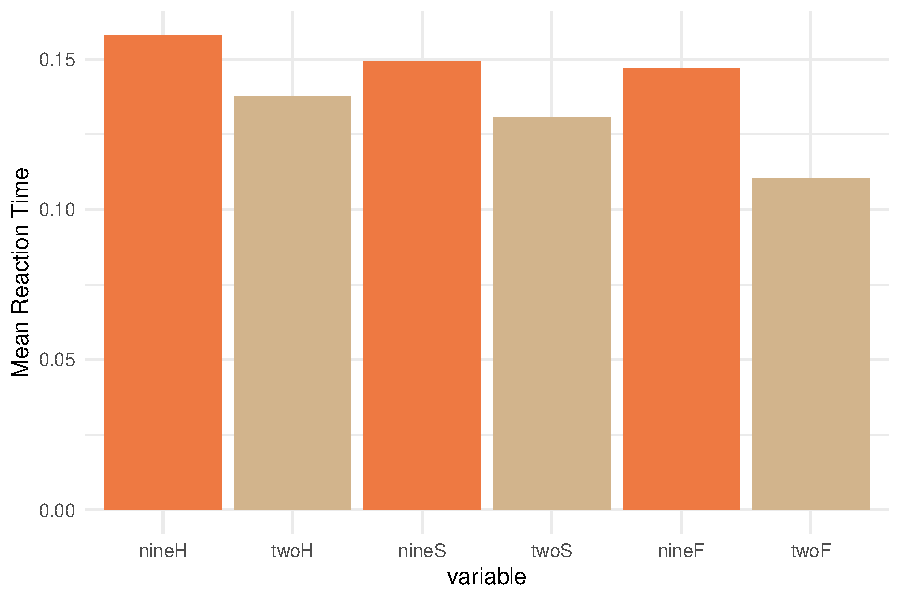
\includegraphics{2019vs2022BarGraph}
  \caption{The reaction times from 2019 and 2022 World Track and Field
  Championship. ``H'', ``S'', and``F'' refer to the heats, semifinals, and finals
  respectively.}
  \label{fig:2019vs2022Graph}
\end{figure}
\of{I included this here for now, but feel free to change the location.  I will
add references to it and explanation of it along with some descriptive statistics about
the size and mean/median,std dev, size of the data.}
\jy{Show dot plots which would give the distribution; without uncertainty
  measure, the mean does not tell much.}


\section{Methods} \label{sec:Methods}

The data described in Sections~\ref{sec:dataworld} and~\ref{sec:databeyond} were
analyzed with GLMM and rank-based methods, respectively.


\subsection{GLMM}\label{sec:glmm}
Based on an exploratory analysis using the GLMM model for the reaction times
from the World Championships, the final model we chose was a gamma mixed-effect 
model. As suggested by the log-likelihood and the Akaike Information
Criterion (AIC), the normal error model on the log-scale was found to be
much inferior to the gamma model which better captures the skewness of the
data. A random effect for the venue or year was also found to be necessary, 
which makes intuitive sense given the discussion in Section~\ref{sec:dataworld}. 
Let $Y_{ij}$ be the reaction time of observation~$j$ in year~$i$.
%\eds{we know that many of the athletes compete in multiple world championships,
%  how is this athlete clustering being accounted for here?}
%\jy{We could add an athlete random effect too, if the players are identified in
%  the data.}
%\jy{Owen, do we have athlete id in the data?}
Conditional on a venue effect $z_i$ of year~i,  $Y_{ij}$ is modeled by 
gamma distribution. In the classic generalized linear model (GLM) sense,
$Y_{ij}$ has conditional mean
\[
g\{E(Y_{ij} | z_i)\} = \alpha + z_i,
\]
and dispersion parameter $\phi$, where $g$ is a known link function and
$z_i$ is a normally distributed random effect with mean zero and
variance~$\sigma^2$. Although \citet{lo2015idlink} suggested that the gamma 
family with an identity link works well for reaction time data, the logarithm 
link function worked better for our data and additionally ensures the positivity
of the conditional mean. The gamma mixed-effect model can be fit with the 
\texttt{glmer()} function in R package \texttt{lme4} \citep{lme4}.


To better understand this model, we can identify the gamma model in terms of the
commonly used shape and scale parameters. For a gamma distribution with
shape~$a$ and scale~$b$, we have mean $\mu = ab$ and variance $v = ab^2$. The
variance as a function of the mean $\mu$ in the GLM sense is
$v(\mu) = \mu^2 / a$, which implies that the dispersion parameter is
$\phi = 1 / a$. Therefore, for the gamma mixed-effect model, the conditional
gamma distribution of the reaction time $Y_{ij}$ given the venue effect $z_i$
has shape $a = 1 / \phi$ and scale $b = g^{-1}(\alpha + z_i) \phi$. The marginal
distribution of $Y_{ij}$ is a scale-mixture of gamma distributions, which can be
easily simulated from once the parameters are estimated. Many
random numbers generated from the fitted mixture distribution can be used to
approximate the probability of observing a reaction time faster than any given
threshold.  We are specifically interested in the probability of a reaction time
 being less than 0.1 seconds in order to gauge if that is a reasonable 
disqualification barrier.

Finally, we remark here that it is also possible to include a heat or race 
\eds{heat? when I first read this, I thought you meant race as in ethnicity}
\of{Yes I think heat or batch effect works better, especially now that I have
removed most talk about heat from the data section} 
\eds{I see, I did not understand this to be Batch effect when I read it the 
first time.  I commented out the Batch text in the Data section - I think it is 
fine to just discuss it here, as it ultimately was not used.  I will defer to 
Dr Yan on this, however.}
effect to account for some heats possibly having faster or slower 
reaction times for everyone involved in the heat.

Although it is possible that one athlete reacting faster could lead to others reacting
similarly, this does not make much practical sense as the difference between
heats that had fast and slow reaction times are all within 0.12 seconds of each
other. 
\eds{Did you try it and find that the effect was not needed?  If yes,
I would include that here.  That argument 
would be more compelling for its non-use than its difficulty in interpretation.}
\of{We found that including the race effect resulted in the venue effect not
being significant, and thus Prof Yan suggested that we don't include it.  I am
wondering if this is even worth mentioning? Prof Yan, what do you think?} 
\jy{We can revisit the results. It is not surprising that venue effect is no
  longer significant after the batch effect was included. We could do the same
  analysis with the batch-random-effect model.}

\subsection{Rank-based Comparison}\label{sec:rank}


To test the conjecture that the 2022 World Championships timing device may have 
led to faster recorded reaction times, we compare the reaction times of the same
athletes who have attended both the 2022 World Championships and other 
competitions. 
In this setting, we have clustered data with subunit grouping. In particular,
each athlete is a cluster and the multiple reaction times from the same athlete
can be from either the 2022 World Championships or otherwise.
Let $X_{ij}$ be the $j$th reaction time of athlete~$i$, $i = 1, \ldots, n$,
$j = 1, \ldots, m_i$ where $m_i$ is the number of observations from
athelete~$i$. Let $\delta_{ij}$ be the group indicator of $X_{ij}$; $\delta_{ij}
= 1$ if $X_{ij}$ is in group~1 (2022 World Championships) and $\delta_{ij} = 0$ 
otherwise. Athletes are
assumed to be independent, while subunit observations from the same athlete are
not. The null hypothesis $H_0$ to be tested is that there is no difference
between the two groups; i.e., the distribution of $X_{ij}$ remains the same
regardless of the group indicator $\delta_{ij}$.


\citet{datta2005rank} proposed an extension of the Wilcoxon rank-sum test to
clustered data with subunit-level grouping. The test is designed based on a
within-cluster resampling principle. Consider randomly picking one observation
from each cluster to form a pseudo-sample. Let $X_i^*$ be a random pick from the
$i$th cluster in the pseudo-sample and $\delta_i^*$ its group indicator. The
Wilcoxon rank-sum statistic for the pseudo-sample is
\[
W^* = \frac{1}{n + 1} + \sum_{i=1}^{n} \delta_{i}^{*} R_{i}^{*},
\]
where $R_{i}^{*}$ is the rank of $X_{i}^{*}$ in the pseudo-sample.
The test statistic $S$ is the average of $W^*$ averaged over all possible
pseudo-samples conditioning on the observed data and group indicators.
The mean and variance of $S$ under $H_0$ can be derived so that $S$ can be
standardized to form a statistic $Z$ which follows standard normal distribution
asymptotically \citep[p.910]{datta2005rank}. An implementation of this method is
available from the \texttt{clusWilcox.test()} function with
\texttt{method = `ds'} from R package \texttt{clusrank}
\citep{jiang2017wilcoxon}.
\eds{are you including preliminary heat data as possible within cluster 
observations in this analysis?  Based on your 
discussion in Section 2.1 about how they are not comparable, it may not be fair 
to include them here?  Or perhaps do the analysis with and without prelim heat
data to see if it makes a difference?}
\of{Yes I am including prelminary heat data.  The primary reason is that there
would be few datapoints otherwise.  I ran the numbes without prelims, the number
of observations dropped from 65 to 26 and the number of clusters from 15 to 9, the
p value increased from 0.000155 to 0.007332.
The calculations are at the bottom of RankComparison.Rmd}


\section{Results} \label{sec:Results}

\subsection{GLMM} \label{subsec:Results_GLMM}

\jy{motivate first why you want to run the analysis with and without the 2022 data.}

\of{Add something like this to the start of the paragraph?}
We may want to consider analyzing all four data sets separately because
comparing the model based on all the data to the model based on data excluding 
2022 can provide an indication about the impact of the 2022 data.
We hope to see that by including 2022 data,
the probability of observing a significantly low reaction time increases. 
Table~\ref{tab:Gamma_parameters} summarizes the results from the gamma model 
from different data sets and shows the standard error of the year
effect increases for both the men's final and men's pooled data sets when
including 2022.  The men's final data venue effect error increased from 0.439
to 0.504 and from 0.0495 to 0.0554 for the men's pooled data.  This demonstrates
that the inclusion of 2022 increased the randomness of the data and motivates
the rank-based study (see Section~\ref{subsec:Results_Rank}).

\jy{Close captions with a period.}
\begin{table}
  \centering
  \caption{Summary statistics for the GLMM on various data sets.} 
  \begin{tabular}{c c c c c c}
      \toprule
      Dataset & Venue standard error & Int effect est & Int se & Int var & Resid Var \\
      \midrule
      Old Finals & 0.0439 & $-1.901$ & 0.0251 & 0.0019 & 0.0109 \\
      All Finals & 0.0504 & $-1.914$ & 0.0280 & 0.0025 & 0.0112 \\
      Old Pooled & 0.0495 & $-1.853$ & 0.0305 & 0.0024 & 0.0243 \\
      All Pooled & 0.0554 & $-1.869$ & 0.0348 & 0.0031 & 0.0235 \\
      \bottomrule
  \end{tabular}
  \label{tab:Gamma_parameters}
\end{table}


\jy{label the table and reference to it; clean it up}
\begin{table}
  \centering
  \caption{Probabilities of observing reaction times less than 0.1, 0.08, and
  0.08 for various data sets.}
  \begin{tabular}{c c c} 
   \toprule
   Data Set & P(RxnTime $<$ 0.1) & P(RxnTime $<$ 0.08) \\ 
   \midrule
   Old Finals & $4.39\cdot10^{-4}$ & $2.0\cdot10^{-5}$ \\
   All Finals & $8.56\cdot10^{-4}$ & $6.0\cdot10^{-7}$ \\
   Old Pooled & $5.76\cdot10^{-3}$ & $1.0\cdot10^{-4}$ \\ 
   All Pooled & $6.86\cdot10^{-3}$ & $1.3\cdot10^{-4}$ \\
   \bottomrule
  \end{tabular}
  \label{tab:Sim_probability}
\end{table}

\begin{table}
  \centering
  \caption{Suggested reaction time barriers based on probability of observing
  a time less the barrier. \of{Not sure if this makes sense}}
  \begin{tabular}{c c c} 
   \toprule
   Data Set & P(RxnTime $<$ x = .001) & P(RxnTime $<$ x = 0.0001) \\ 
   \midrule
   Old Finals & $0.103$ & $0.095$ \\
   All Finals & $0.101$ & $0.093$ \\
   Old Pooled & $0.090$ & $0.080$ \\ 
   All Pooled & $0.089$ & $0.079$ \\
   \bottomrule
  \end{tabular}
  \label{tab:Sim_time}
\end{table}


Using the gamma function with link set to log, the probability of the reaction 
time being less than 0.1 seconds can be calculated to see if Allen's 
disqualification was an anomaly as described in Section~\ref{sec:glmm}.
Calculations were performed in R using the methods described in 
section~\ref{sec:glmm} with the use of the \citet{lme4} package.


At a size of $n=10,000,000$, \eds{use different letter as $n$ was already used 
for number of athletes, $B?$} \of{Could I just say "At a size of 10,000,000"? 
Otherwise I am fine with using "B" instead of "n"} \eds{we may have lost the 
rest of this sentence?}


The calculated probabilities of a reaction time 
being below 0.1 seconds for the various different data sets are shown in 
Table~\ref{tab:Sim_probability}. Prior to the 2022 World Championships, there 
was a 0.0439\% chance (based on the
simulated results) of observing a reaction time below 0.01 seconds in the men's
finals.
That means that we would expect a time below the threshold to occur
once every 2,277 starts.  Considering there are roughly 8 men's finals reaction
times every 2 years (the World Championships are biennial), every 569 years there
should be a time as extreme as Allen's. This seems extremely unlikely, and thus
it seems like there may be an additional explanation for the fast reaction times.


When the 2022 data is included in the analysis, it is interesting that the 
probability of observing a reaction time below 0.1 seconds increases drastically 
for the finals data and increases by a smaller margin for the pooled data.  By
including 2022 in the data, the chances of observing an extreme time are 
increased, suggesting that 2022 is a high outlier for reaction times compared to
 other years.


Table~\ref{tab:Sim_probability} also shows that changing the reaction time 
barrier from 0.1 seconds to 0.08 seconds drastically reduces the chances of 
observing a reaction time that would break the barrier.  For the dataset of all 
finals data, the probability
associated with observing a reaction time below 0.08 seconds was $6\cdot10^{-7}$.
If IAAF \eds{or World Athletics?} were to change the reaction time the way that 
\citet{komi2009iaaf}
suggests, the probability would be so much lower that athletes would likely not
have a case to make when arguing against a disqualification.

We can use the same model but alter our interpretation slightly to select a 
reaction time barrier given the probability of observing a time less than the 
barrier.  For example, if we want a 0.1\% chance of observing an illegally fast 
reaction time for the men's pooled dataset that includes 2022, then the reaction
time barrier should be 0.089 seconds, as shown in Table~\ref{tab:Sim_time}.  We
can repeat this calculation for each dataset and for various probability levels,
for example a probability of 0.0001 (one disqualification for every 10,000 starts)
results in a reaction time barrier of 0.079 for the men's pooled dataset.  
Tables~\ref{tab:Sim_time} shows that the inclusion of 2022 results in a lower
reaction time barrier, further showing the claims above that the reaction times
in 2022 were low.

%Discussion should show that random effect
%and standard error increase and that 2022 is special.  Now talk about Seiko
%timing equipment

%Citation needed in this section
Since 1985 Seiko Holding Corporations has served every World Athletics 
Championships as the official timer \citep{wa2022seiko}.  Since 1985, the 
technology and the ability
to accurately predict measurements: long jump distances, false starts, total 
time, reaction time, etc. have all dramatically improved.  Seiko did not start 
tracking reaction time as an official measurement until 1999 in the men's and 
women's 100 meter \eds{110 for men?} hurdles. 
Seiko regularly updates their equipment so that they provide cutting edge
technology to the World Track and Field Championships, the highest stakes in the 
world of running outside of the Olympics. Seiko's technology for detecting 
reaction times relies on the pressure that athletes exert on the plate when they 
push off.  Their systems measure the time differential
between when the ``gun" goes off to start the race and when the pressure changes 
\citep{wa2022seiko}.  If an athlete has a reaction time under 0.1 seconds, it 
is deemed a 
false start as it is considered that no athlete can react so quickly 
\citep{Seiko-Timing}.  Thus, a reaction time of for example 0.05, suggests that 
the athlete predicted the gun and it was luck that caused their abnormally high 
time.  At the World Championships level, World Athletics and Seiko want to remove 
that element of luck and thus impose the 0.1 second barrier. In 2013, Seiko 
upgraded their timing equipment for sprinting events (110 meter hurdles falls 
under this category) \citep{wa2013backtage}. Since 1999, the
slowest reaction 
times in the men's 110-meter hurdle were recorded in 2013.  That is not to say
 that the higher 
times were caused by Seiko's equipment, but the two may be related.  It is worth 
noting that prior
to 2022, Seiko again upgraded its technology but for its jump management system.
\eds{I would argue that this paragraph should go in the discussion as there are 
no results presented here}

\subsection{Rank-based Comparison} \label{subsec:Results_Rank}

\jy{Remind the readers what the analysis was about: two-group comparison with
  group being ....}

The rank based methods described in Section~\ref{sec:rank} are used
to determine if the reaction times for athletes who had competed at other 
championships differed significantly from the 2022 World Championships.  We can
use the 2019 World Championships and the 2022 national-level championships as a 
precedent to see how athletes performance changed across different championships.


When the clusrank rank sum test was performed, the ``ds" method produced a z score of
2.9751 and p value of 0.001464.  \eds{what is the ds method?} 
This value is for a one-sided test and show that
the mean reaction time on average in 2019 was larger (slower) than the mean 
reaction time
in 2022 for athletes who competed in both championships at an alpha level of 0.01.
This provides good evidence that athletes who competed in both 2019 and 2022 got
faster during that timespan.  \eds{That is not the only explanation}


Repeating the data collection steps and
again performing a clustered analysis for a Wilcoxon ranked sum test
results in two new z scores and p values. 
\eds{I am not sure why you are repeating the data collection steps and
again performing a clustered analysis here.  Also, if there are two new z-scores
and p values, why are you only reporting one?}
  The ``ds" method produced a z score of
3.6069 and p value of 0.000155. This result is highly significant and shows that
the times at the national stage of competition were significantly higher than
the reaction times at the World Championships even for an alpha level of 0.001.

\eds{also consider moving the following paragraph to discussion??}
As Seiko timed both events, there should not be a significant
difference if the timing equipment in both instances was working correctly.
\eds{you just mentioned in the last subsection that Seiko upgraded its 
technology prior to 2022}
  To put it simply, there is not a reasonable explanation for 
this. It is inconceivable that so many athletes would improve such a significant
amount in such a small amount of time. Six countries are represented in this 
comparison, which drastically decreases the chances of this issue being caused by
one specific country.  The United States athletes' improvement in times was
discussed earlier in the paper, but this data shows that on average there was
\jy{any reference?}
improvement for British, Polish, French, Brazilian, and Spanish athletes.


\section{Discussion}\label{sec:Discussion}

One conclusion from the analysis in \citet{zhang2021correlation} was that 
athletes'
reaction times improved from 2011 to 2019.  However this study does not consider 
data from 1999 to 2009, and over this timespan athletes get slower and then
faster.  Figure~\ref{fig:Boxplots} shows that for the men's pooled data, the 
year with the fastest median reaction time before 2022 was 1999.  Thus, this 
reject's Zhang et al.'s conclusion that athletes are getting faster because they 
were 
fast over twenty years ago. One possible explanation for why 2011 had such
high variation was because of the IAAF rule discussed earlier that increased the
penalty of a false start to an instant disqualification \citep{iaaf2009falsestart}.
Athletes may have been overly cautious to false start and may have consciously
or sub-consciously reacted slower as a result.  Instead, a more appropriate 
conclusion may be that there is a lot of variability in reaction times and that
the context behind the races matters.

It is worth noting that in the semifinals of the 2022 World Track and
Field Championships, Allen's reaction time was 0.101 which is only 0.001 above
the legal limit. What this suggests is that Allen may have strong reflexes
and be able to react extremely well to the sound of the gun. It seems unlikely 
that Allen would be able to correctly predict the gun with such precision two 
times in a row, which is the exact reason that the 0.1 second reaction time 
disqualification barrier was
imposed in the first place. Thus having a quick reaction time multiple times
may indicate skill rather than luck. Devon 
Allen is a very good athlete, as evidenced by his football career at the 
University of Oregon
and making it onto the Philadelphia Eagles practice squad this past year 
\citep{hurley2022eagles}. The 0.099 reaction time may not have been 
a product of Devon Allen predicting the start of the race but rather a 
combination of a quick reaction and a possibly faulty sensor.

Devon Allen's disqualification at the World Track and Field Championships was
possibly the result of both a faulty timing equipment and Devon Allen
reacting extremely quickly to the start.  Our analysis showed that
the 2022 World Track and Field Championships were a low outlier compared to
every other year in terms of average reaction time.  Additionally, it was shown
through a gamma mixed effects model that there are significant year and race
effects \eds{remove race effects?} that greatly impact reaction time.  

%\eds{I would suggest removing the last two sentences, as they would suggest your
% modeling with GLMM is not good}.  
%\of{I agree and they have been removed}

This paper does not consider data from the women's 100 meter hurdle, and although
that was initially because of concerns over reaction time differences in men and
women, exploratory analysis showed that 2022 was at best only
slightly faster relative to other championships going back to 2003 
\eds{check year}. \eds{this seems to contradict the Robert Johnson conclusion in 
the intro, unless he only considered sprint and not hurdles?} Likewise,
the rank-based comparisons resulted in p values that were not significant.  The
lack of evidence from the women's data makes it harder to conclude 
that the sensors used at the 2022 championships were faulty, although it is
unknown if the sensors for the men's 110 meter hurdle and women's 100 meter
hurdle were the same.

Thus while it seems easy
to conclude that Devon Allen was wrongly disqualified, that may not necessarily
be the case. 
If there are issues with reaction time such as athletes approaching 
the 0.1 
second barrier again at the next World Championships (August 2023), then 
World Athletics 
needs to adjust that threshold and allow for faster reaction times so that 
athletes with superb 
reflexes are not penalized. %like how Allen was in 2022.  
World Athletics did not
do anything in response to the \citet{komi2009iaaf} study, but perhaps they 
should now so
that the story of Devon Allen is not repeated.

\section*{Appendix}
\label{sec:Appendix}
%Put downloadable data spreadsheet
The World Championships data are available from the World Athletics website:
\url{https://www.worldathletics.org/results/world-athletics-championships}.

\jy{You have countries beyond United States}
The United States Track and Field Championships data are available at: 
\url{https://www.flashresults.com/2022_Meets/Outdoor/06-23_USATF/}



\jy{Go over the references to see clues to clean in the bib source}
\bibliographystyle{chicago}
\bibliography{citations.bib}


\end{document}

Here are important statistics grouped by both model and data set:
All Men final's Data
\begin{center}
  \begin{tabular}{|c | c | c | c | c | c | c |} 
   \hline\hline
   Model & AIC & Log Likelihood & Int effect est & Int se & Int var & Resid Var \\ [0.5ex] 
   \hline
   linear one & -472.7 & 238.3 & 0.1484 & 0.0019 & N/A & N/A \\ 
   \hline
   linear year & -468.7 & 237.4 & 0.1481 & 0.0030 & 7.762e-05 & 2.457e-04 \\
   \hline
   men finals one gamma & -477.3 & 240.7 & 6.738 & 0.0844 & N/A & N/A \\
   \hline
   men finals year gamma & -491.1 & 248.5 & 6.8121 & 0.1895 & 0.1148 & 0.0112 \\
   \hline
   men finals one gamma log & -477.3 & 240.7 & -1.908 & 0.0125 & N/A & N/A \\
   \hline
   men finals year gamma log & -491.0 & 248.5 & -1.914 & 0.0280 & 0.0025 & 0.0112 \\ [0.5ex]
   \hline
  \end{tabular}
\end{center}

Pre-2022 final's data
\begin{center}
  \begin{tabular}{|c | c | c | c | c | c | c |} 
   \hline\hline
   Model & AIC & Log Likelihood & Int effect est & Int se & Int var & Resid Var \\ [0.5ex] 
   \hline
   linear one & -450.7 & 227.4 & 0.1495 & 0.0019 & N/A & N/A \\
   \hline
   linear year & -444.1 & 225.0 & 0.1496 & 0.0028 & 5.691e-05 & 2.470e-04 \\ 
   \hline
   gamma one & -455.8 & 229.9 & 6.687 & 0.0834 & N/A & N/A \\
   \hline
   gamma year & -465.1 & 235.5 & 6.714 & 0.1674 & 0.0859 & 0.0109 \\
   \hline
   gamma one log & -455.8 & 229.9 & -1.900 & 0.0125 & N/A & N/A \\
   \hline
   gamma year log & -465.0 & 235.5 & -1.901 & 0.0251 & 0.0019 & 0.0109 \\ [0.5ex]
   \hline
  \end{tabular}
  \end{center}

All Men's semifinal and finals data
\begin{center}
  \begin{tabular}{||c | c c c | c c c||} 
   \hline
   Athlete & United States H & United States S & United States F & World H & World S & World F \\ [0.5ex] 
   \hline\hline
   Devon Allen & 0.201 & 0.153 & 0.160 & 0.123 & 0.101 & 0.099 \\ 
   \hline
   Trey Cunningham & 0.186 & 0.185 & 0.182 & 0.115 & 0.120 & 0.109 \\
   \hline
   Grant Holloway & 0.192 & 0.190 & N/A & 0.147 & 0.128 & 0.124 \\
   \hline
   Daniel Roberts & 0.181 & 0.200 & 0.183 & 0.179 & N/A & N/A \\ [0.5ex]
   \hline
  \end{tabular}
  \end{center}

Pre-2022 Men's semi finals and finals data
\begin{center}
  \begin{tabular}{|c | c | c | c | c | c | c |} 
   \hline
   Model & AIC & Log Likelihood & Int effect est & Int se & Int var & Resid Var \\ [0.5ex] 
   \hline\hline
   linear one & -1539 & 771.5 & 0.1544 & 0.0015 & N/A & N/A \\
   \hline
   linear year & -1564 & 785.4 & 0.1562 & 0.0037 & 1.280e-04 & 6.273e-04 \\ 
   \hline
   gamma one & -1626 & 814.9 & 6.475 & 0.0608 & N/A & N/A \\
   \hline
   gamma year & -1688 & 846.8 & 6.426 & 0.1923 & 0.0989 & 0.0243 \\
   \hline
   gamma one log & -1626 & 814.9 & -1.868 & 0.0094 & N/A & N/A \\
   \hline
   gamma year log & -1687 & 846.6 & -1.853 & 0.0305 & 0.0024 & 0.0243 \\ [0.5ex]
   \hline
  \end{tabular}
  \end{center}



Sorted By Model instead:
Linear Model with no venue effect
\begin{center}
  \begin{tabular}{|c | c | c | c | c | c | c |} 
   \hline
   Dataset & AIC & Log Likelihood & Int effect est & Int se \\ [0.5ex] 
   \hline\hline
   All Finals & -472.7 & 238.3 & 0.1484 & 0.0019 \\
   \hline
   Older Finals & -450.7 & 227.4 & 0.1495 & 0.0019 \\ 
   \hline
   All Pooled & -1667 & 835.5 & 0.1529 & 0.0014 \\
   \hline
   Older Pooled & -1539 & 771.5 & 0.1544 & 0.0015 \\
   \hline
  \end{tabular}
  \end{center}

Linear model with venue effect
\begin{center}
  \begin{tabular}{|c | c | c | c | c | c | c | c |} 
   \hline
   Dataset & AIC & Year se & Log Likelihood & Int effect est & Int se & Int var & Resid Var \\ [0.5ex] 
   \hline\hline
   All Finals & -468.7 & 0.0088 & 237.4 & 0.1481 & 0.0030 & 7.762e-05 & 2.457e-04 \\
   \hline
   Older Finals & -444.1 & 0.0075 & 225.0 & 0.1496 & 0.0028 & 5.691e-05 & 2.470e-04 \\ 
   \hline
   All Pooled & -1713 & 0.131 & 859.3 & 0.1541 & 0.0040 & 1.719e-04 & 5.926e-04 \\
   \hline
   Older Pooled & -1564 & 0.113 & 785.4 & 0.1562 & 0.0037 & 1.280e-04 & 6.273e-04 \\
   \hline
  \end{tabular}
  \end{center}

Gamma model with venue effect
\begin{center}
  \begin{tabular}{|c | c | c | c | c | c | c | c |} 
   \hline
   Dataset & AIC & Year se & Log Likelihood & Int effect est & Int se & Int var & Resid Var \\ [0.5ex] 
   \hline\hline
   All Finals & -491.1 & 0.3388 & 248.5 & 6.8121 & 0.1895 & 0.1148 & 0.0112 \\
   \hline
   Older Finals & -465.1 & 0.2930 & 235.5 & 6.714 & 0.1674 & 0.0859 & 0.0109 \\ 
   \hline
   All Pooled & -1848 & 0.3612 & 926.9 & 6.553 & 0.2269 & 0.1305 & 0.0234 \\
   \hline
   Older Pooled & -1688 & 0.3145 & 846.8 & 6.426 & 0.1923 & 0.0989 & 0.0243 \\
   \hline
  \end{tabular}
  \end{center}

Gamma model with venue effect and link=log
\begin{center}
  \begin{tabular}{|c | c | c | c | c | c | c | c |} 
   \hline
   Dataset & AIC & Year se & Log Likelihood & Int effect est & Int se & Int var & Resid Var \\ [0.5ex] 
   \hline\hline
   All Finals & -491.0 & 0.0504 & 248.5 & -1.914 & 0.0280 & 0.0025 & 0.0112 \\
   \hline
   Older Finals & -465.0 & 0.0439 & 235.5 & -1.901 & 0.0251 & 0.0019 & 0.0109 \\ 
   \hline
   All Pooled & -1848 & 0.0554 & 927.0 & -1.869 & 0.0348 & 0.0031 & 0.0235 \\
   \hline
   Older Pooled & -1687 & 0.0495 & 846.6 & -1.853 & 0.0305 & 0.0024 & 0.0243 \\
   \hline
  \end{tabular}
  \end{center}
